
\providecommand{\main}{..} 
\documentclass[\main/notes.tex]{subfiles} 

\begin{document} 
\begin{center} 
\textbf{{\Large One-Zone Models}} 
\end{center} 

\noindent 
{\Large \textit{The Impact of the AGB Star Yields}} 
\par\noindent 
\textbf{How do the abundances predicted by one-zone models differ between 
the~\citet{Cristallo2011} and~\citet{Karakas2010} yield sets?} 
\par\noindent 
Taking~$\dot{M}_\star$ = constant,~$\eta$ = 2.0, and~$y_\text{N}^\text{CC}$ = 
$4.15\times10^{-4}$ as suggested by supernova yields and the observed 
[N/O] plateau at low [O/H], the [N/O]-[O/H] tracks for~$\tau_\star$ = 1, 2, 4, 
and 8 Gyr for both studies is shown in Fig.~\ref{fig:onezone_cristallo_karakas}. 
The black dotted line denotes the population-averaged trend published 
in~\citet*{Henry2000}. 
The model recovers the qualitative observational trend with 
the~\citet{Cristallo2011} yields, though the increase in [N/O] at high [O/H] 
isn't as large as in the observations. 
The~\citet{Karakas2010} yields predict a trend in tension with the observations, 
but this makes sense when considering how these yields depend on mass and 
metallicity (see Fig.~\ref{fig:n_agb_yields}). 
Their highest yields are for higher mass stars at low metallicity; although 
the~\citet{Cristallo2011} yields also predict the yields to increase with 
stellar mass, the metallicity trend appears to be what's most important here. 
At early times when [O/H] is low, the high mass AGB stars dump a lot of N, 
getting the ISM off the plateau more or less immediately. 
The peak and subsequent decrease in [N/O] at high [O/H] can be understood from 
the decrease in the N yields near solar Z as reported by~\citet{Karakas2010}. 

\begin{figure*} 
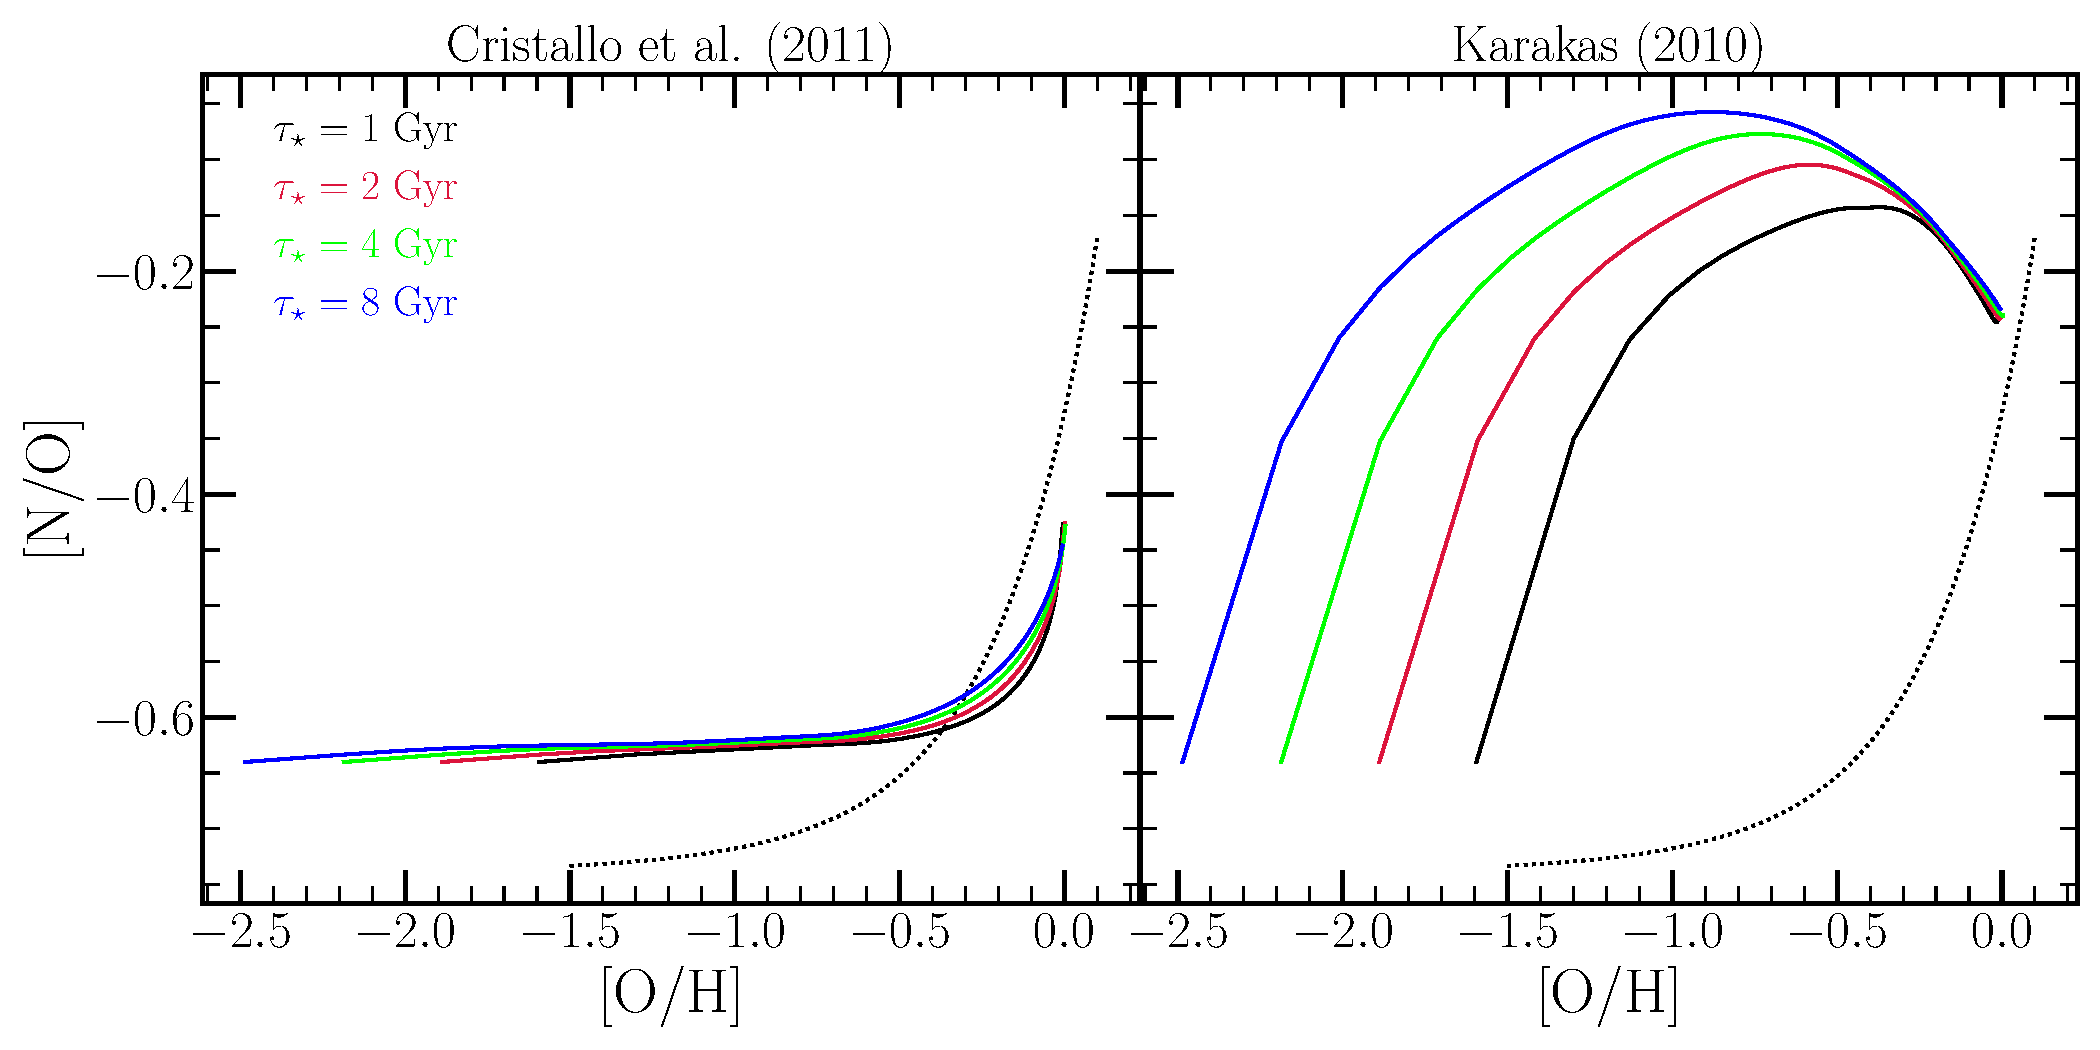
\includegraphics[scale = 0.45]{\main/onezone/onezone_cristallo_karakas.pdf} 
\caption{[N/O]-[O/H] tracks as predicted by~\citet{Cristallo2011} (left) 
and~\citet{Karakas2010} (right). } 
\label{fig:onezone_cristallo_karakas} 
\end{figure*} 

Since the~\citet{Cristallo2011} yields recover the correct trend, but 
the~\citet{Karakas2010} yields appear to have a more realistic magnitude, 
better agreement with the observations can be achieved by simply amplifying 
the~\citet{Cristallo2011} yields by some factor; this is demonstrated in 
Fig.~\ref{fig:onezone_cristallo}. 
The model with amplified yields agrees with the observational result better, 
even though it overestimates [N/O] and all [O/H]. 
A better match could be achieved by lowering~$y_\text{N}^\text{CC}$, which 
predicts a plateau at a marginally higher [N/O] than~\citet*{Henry2000}. 
Nonetheless, this is a good demonstration that even taking the more realistic 
of the two yield sets, the yields must be artificially amplified by a 
substantial prefactor in order to predict~$\sim$solar [N/O] at~$\sim$solar 
[O/H]. 
\textbf{
This re-raises the question of the timescales of N enrichment from a 
single stellar population: if AGB stars make up a more substantial fraction 
of the nitrogen enrichment in the universe, will that increase the 
characteristic delay times of nitrogen production seen with the base set of 
yields from~\citet{Cristallo2011}?
This should impact the amplitude of variability in its production. 
} 

\begin{figure*} 
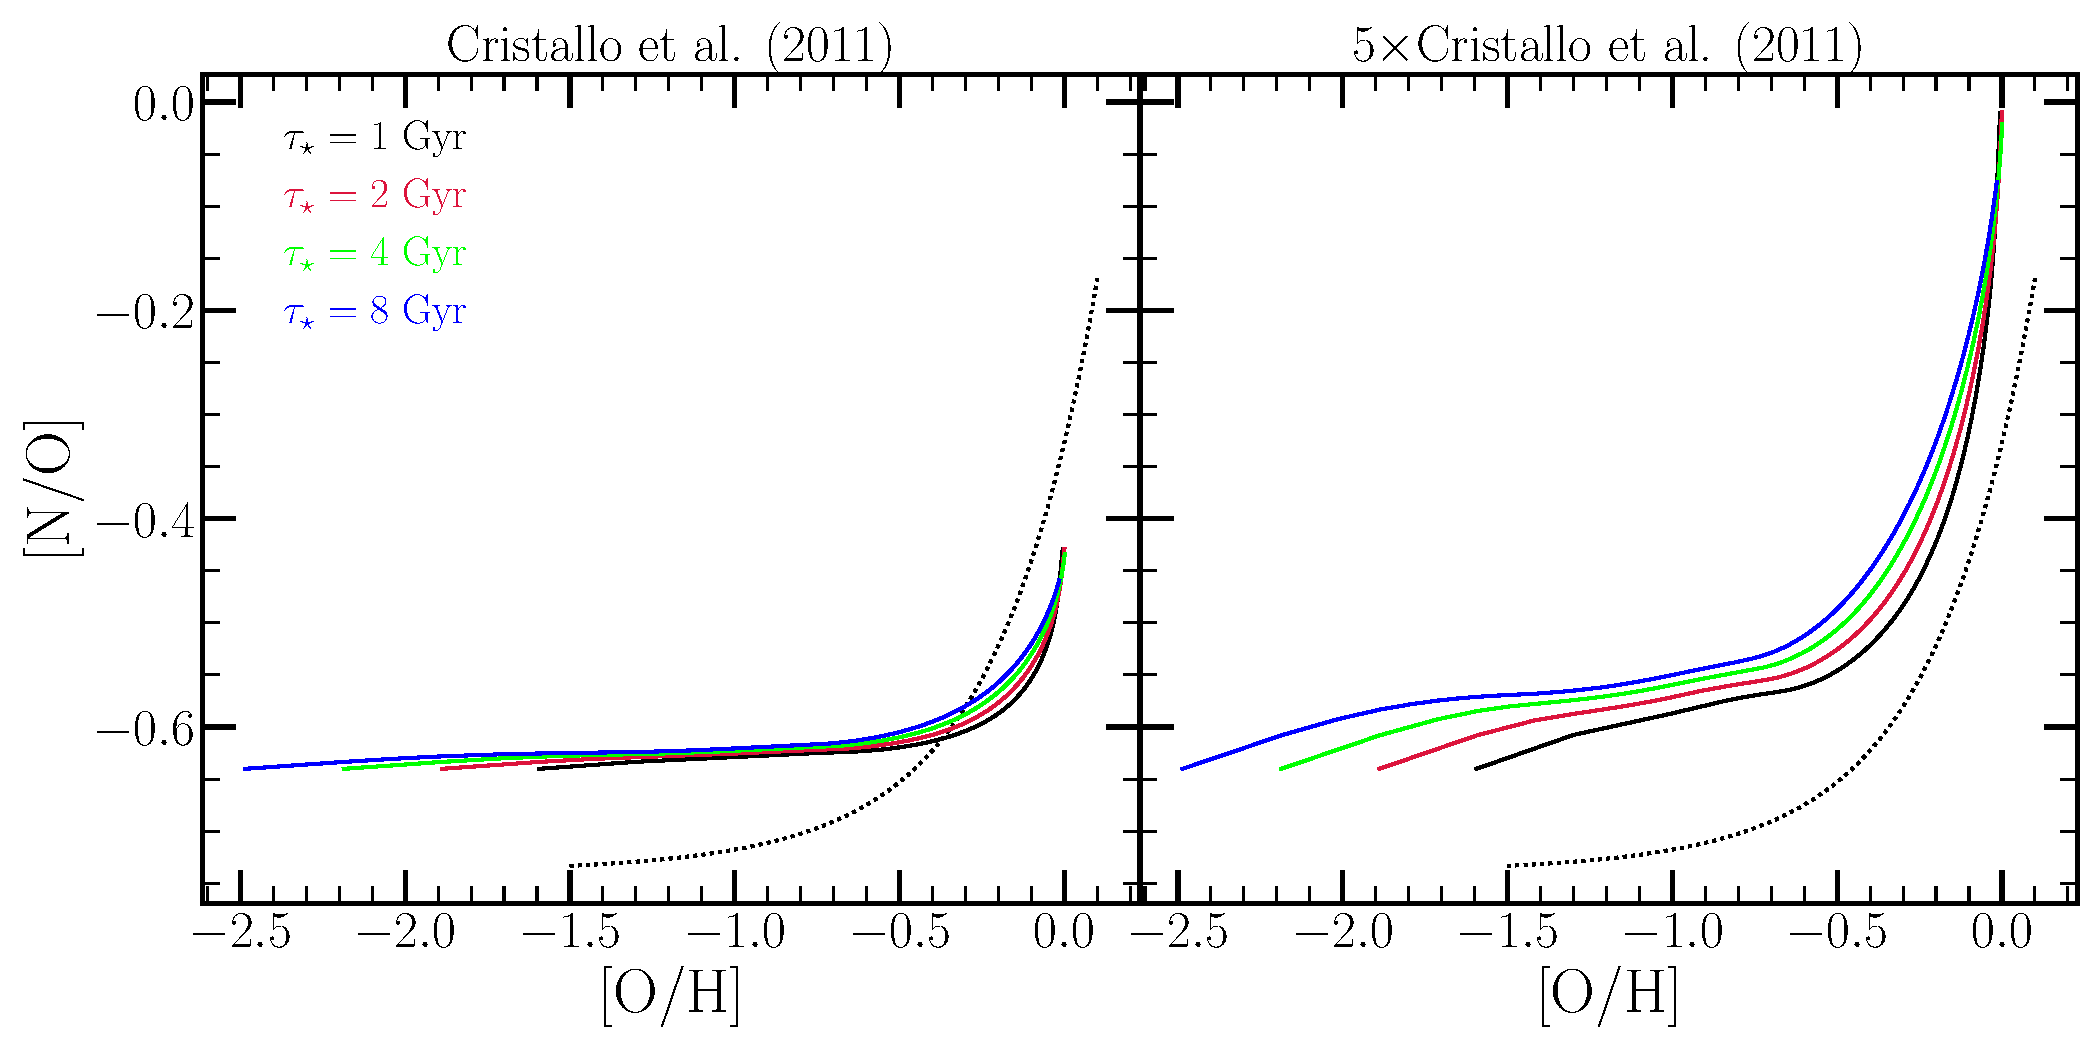
\includegraphics[scale = 0.45]{\main/onezone/onezone_cristallo.pdf}
\caption{[N/O]-[O/H] tracks as predicted with the~\citet{Cristallo2011} 
yields (left), and with the same yield set but amplified by a factor of 5 
(right). }
\label{fig:onezone_cristallo} 
\end{figure*} 

\biblio 

\end{document} 
